\documentclass[a4paper,12pt]{article}

	\usepackage{amssymb,amsfonts,amsmath,amsthm}	% математические дополнения от АМС
	\usepackage{graphicx}
	\usepackage{tabularx}
	\usepackage{hyperref}
	\usepackage{textcomp}
	\usepackage{xcolor}
	
	\usepackage{graphicx}
    \usepackage{subcaption}

	
	\usepackage[utf8x]{inputenc}
	\usepackage[T1,T2A]{fontenc}
	\usepackage[russian]{babel}

	\linespread{1.3}					    % полуторный интервал
	\frenchspacing

%===============================   #Alias   ====================================

%===============================================================================	
	%\hfuzz=0.5pt
	%\tolerance=3000

	\title{Практический семинар\\ \huge{Визуализация структур в UCSF Chimera}}
	\author{Данила Яковлев}
	\date{2018}

\begin{document}
\maketitle
\begin{abstract}
Количество доступных трехмерных структур биомолекул постоянно увеличивается и современная биохимическая работа все чаще требует не только <<мокрых>> экспериментов, но и анализа структуры изучаемого объекта. При этом, наглядное представление трехмерных объектов на бумаге~-- задача не всегда тривиальная. Хорошая картинка может существенно сократить текст статьи, а плохая~-- наоборот, запутать читателя. 
\end{abstract}

Практический семинар <<Визуализация структур в UCSF Chimera>> длительностью 2 академических часа поможет студентам научиться подготавливать качественные иллюстрации для научных работ. На семинаре будут рассмотрены основные приемы работы с программой UCSF Chimera\footnote{\url{https://www.cgl.ucsf.edu/chimera/}}:
\begin{enumerate}
    \item различные форматы файлов со структурами белков и ДНК; % +
    \item где их можно получить и как открыть в химере; % +
    \item освещение (одно-, двух- и трехточечное, изотропное), цвет фона; % +
    \item способы отображения биомолекул (полноатомный, \textit{ribbon}, поверхности); % +
    \item выделение элементов структуры, именованные группы атомов, отображение/скрытие элементов структуры; % +
    \item структурное выравнивание; % +
    \item раскраска: по атрибутам, радуга; %+
    \item поиск водородных связей и межатомных контактов, построение поверхностей \textit{SAS, SES} и \textit{VdW}; %+
    \item прозрачность, сечения и вид в разрезе; %+
    \item сохранение полученной иллюстрации, виды доступной трассировки лучей.
\end{enumerate}
\hfill
\begin{figure}[h!]
  \includegraphics[width=\linewidth]{Figures/Protein.pdf}
  \caption{\textit{Пример иллюстрации подготовленной с помощью UCSF Chimera.}}
  \label{fig:smug}
\end{figure}\clearpage
\section{Виды структур и как их получить}
Основные форматы структур больших биомолекул~-- PDB и mmCIF. Оба формата текстовые, с определенным 
синтаксисом\footnote{Документация: \url{https://www.wwpdb.org/documentation/file-format}}. 
Формат PDB считается устаревшим, но все еще широко используется. Если вы начинаете новый проект, 
связанный со структурами биомолекул, лучше использовать mmCIF там, где это возможно, так как этот
формат устойчивее к ошибкам и позволяет хранить больше метаданных.

Малые молекулы, например, метаболиты, коферменты и лекарственные препараты тоже можно закодировать в PDB, но еще довольно часто встречаются форматы: \href{https://reference.wolfram.com/language/ref/format/MOL2.html}{MOL2}, \href{http://libatoms.github.io/QUIP/io.html#extendedxyz}{XYZ} и однострочники (\href{http://opensmiles.org/opensmiles.html}{SMILES} и \href{https://pubs.acs.org/doi/pdfplus/10.1021/ci960109j}{SYBYL Line Notation})

Чаще всего, структура, с которой вы работаете, уже содержится в какой-нибудь базе данных и иметь файл с ней необязательно, достаточно знать идентификатор (PDB~ID, например)~-- Химера сама загрузит всю необходимую информацию с сервера БД.

\paragraph{Распространенные базы данных структур биомолекул:}
\begin{itemize}
    \item PDB (\href{https://rcsb.org/pdb}{RCSB}, \href{https://www.ebi.ac.uk/pdbe}{PDBe}, \href{https://pdbj.org}{PDBj})~-- структуры белков;
    \item \href{http://ndbserver.rutgers.edu}{NDB}~-- структуры нуклеиновых кислот;
    \item \href{http://scop2.mrc-lmb.cam.ac.uk}{SCOP2} и \href{http://www.cathdb.info}{CATH}~-- эволюция белков, структурные семейства, домены, ук\-лад\-ка белков;
    \item \href{https://www.ebi.ac.uk/pdbe/emdb/}{EMDB}~-- электронная микроскопия.
\end{itemize}

\paragraph{Базы данных малых молекул}
\begin{itemize}
    \item \href{https://pubchem.ncbi.nlm.nih.gov/}{PubChem}~-- база данных химических соединений от NCBI;
    \item \href{https://www.ebi.ac.uk/chembl/}{ChEMBL} и \href{https://www.ebi.ac.uk/chebi/}{ChEBI}~-- база данных и онтология биомолекул от EBI;
    \item \href{http://zinc15.docking.org}{ZINC}~-- база данных коммерчески доступных соединений (оптимизирована для виртуального скринига);
    \item \href{https://www.ccdc.cam.ac.uk}{CCDC}~-- кембриджская кристаллографическая база данных;
\end{itemize}

\subsection*{Задание~1}
\begin{enumerate}
    \item Запустите Химеру.
    
    \item \textit{Загрузим структуру с сервера PDB:}\\
        В меню\quad\texttt{File~> Fetch by ID...}\quad выберите пункт\quad\texttt{PDB (mmCIF)}, введите \texttt{4MNF}
        и нажмите\quad\texttt{Fetch}.\\
        \textit{Должна открыться структура белка BRAF дикого типа.}
    
    \item \textit{Теперь откроем обычный PDB-файл:}\\
        В меню\quad\texttt{File~> Open...}\quad откройте файл\quad\texttt{braf\_v600e.pdb}.\\
        \textit{К уже открытой структуре белка BRAF WT добавилась структура мутантной формы BRAF V600E.} 
        % PDB ID: 1UWH
        
    \item Выведите список моделей\quad\texttt{Tools~> General Controls~> Model Panel}.\\
        Сколько моделей открыто? Сколько из них активно? Попробуйте скрыть и снова показать модель.
\end{enumerate}

\section{Общие настройки внешнего вида}
По умолчанию структуры в химере рисуются на черном фоне, а иллюстрации для журнала удобнее делать на белом. Быстрее всего поменять фон можно, выбрав одну из предустановленных настроек отрисовки молекул.
\subsection*{Задание~2.1}
В меню\quad\texttt{Presets}\quad выберите пункт\quad\texttt{Publication~1 (silhouette, rounded ribbon)}.\quad Что изменилось? Попробуйте выбрать другие опции.
\subsection*{}
Внешний вид сцены можно настроить более детально:
\subsection*{Задание~2.2}
\begin{enumerate}
    \item В панели\quad\texttt{Actions~> Color~> all options...}\quad измените цвет фона (кнопка\quad\texttt{more...}\quad напротив пункта\quad\texttt{background}) на тот, который вам нравится.
    \item В панели\quad\texttt{Tools~> Viewing controls~> Effects}\quad настройте толщину обводки, тени и затемнение перспективы.
    \item Там же, во вкладке\quad\texttt{Lightning}\quad настройте освещение. Сравните режимы\quad\texttt{Ambient}\quad и\quad\texttt{Two-point}.\quad В чем разница?
    \item В панели\quad\texttt{Tools~> Depiction~> Rainbow}\quad раскрасьте каждую цепь в отдельный цвет.
    \item Скройте все атомы:\quad\texttt{Actions~> Atoms/Bonds~> hide}. Что осталось?
\end{enumerate}
\section{Способы представления молекулы белка}
Во время анализа структуры биомолекулы нас могут заинтересовать разные уровни
организации: от отдельных атомов до межмолекулярных комплексов. Для каждого из уровней удобнее использовать свое представление:
для визуализации активных центров рисовать отдельные атомы, для структуры белка в целом~-- пептидный остов, для белковых
комплексов~-- поверхность доступности растворителя.

\subsection*{Задание~3}
\begin{enumerate}
    \item Выключите отображение остова и включите отображение атомов:\\\quad\texttt{Actions~> Ribbon~> hide}\quad
    $\rightarrow$\\\quad\texttt{Actions~> Atoms/Bonds~> show}.\quad Какие атомы появились? \\
    \textit{Можно сделать картинку не такой шумной:}\\\quad\texttt{Actions~> Atoms/Bonds~> wire}.
    \item Скройте атомы и верните остов.
    \item Постройте поверхность доступности растворителя\\\quad\texttt{Actions~> Surface~> show}.\quad\\ Установите прозрачность поверхности на 50\,\%\\
    \quad\texttt{Actions~> Surface~> transparency~> 50\,\%}.\quad\\Какую информацию может дать о молекуле ее поверхность доступности растворителя?
    \item Закройте поверхности в\quad\texttt{Model Panel (close)}.
\end{enumerate}
\section{Выделение и группы атомов}
Команды, которые мы изучили выше влияют на отображение молекулы в целом. Если же мы хотим поработать только с определенными атомами или остатками, не затрагивая все остальное, то нам нужно будет использовать инструмент <<выделение>> (\texttt{select}).

Выделить интересующие вас атомы и связи можно с помощью мышки, зажав \texttt{Ctrl}. Если выделить за один раз все не получается, выделение можно расширить, зажав \texttt{Shift + Ctrl}.

\subsection*{Задание~4}
\begin{enumerate}
    \item Выделите N-концевые остатки полипептидных цепей (Asp 449 для дикого типа и Asp 447 для V600E).
    
    \item Сделайте выделенные атомы видимыми.
    
    \item Выделите все атомы воды:\quad\texttt{Select > Residue > HOH}\quad
    
    \item Покажите их.
    
    \item Удалите выделенные атомы:\quad\texttt{Actions > Atoms/Bonds > delete}.
    
    \item \textit{Сделаем малые молекулы и ионы видимыми.}\\
    Выделите все нестандартные остатки:\\\texttt{Select > Residue > all nonstandard}
    
    \item Представьте их в виде шариков и палочек:\quad\texttt{Actions > Atoms/Bonds > show $\rightarrow$ ... > ball \& stick}
    
    \item \textit{Оставим в выделении только лиганды.}\\
    Поменяйте режим выделения на вычитание:\\
    \texttt{Select > Selection Mode > subtract}\\
    Уберите из выделения атомы хлора:\\
    \texttt{Select > Residue > CL}
    
    \item Сохраните лиганды в именованную группу:\\
    \texttt{Select > Name Selection ...}\quad введите имя для группы атомов.\\
    Теперь чтобы выбрать именованную группу нажмите\\\texttt{Select > Named Selections > <Имя\_Группы>}
\end{enumerate}
\section{Структурное выравнивание}
Сейчас открытые модели расположены довольно далеко друг от друга и сравнивать их не очень удобно. Чтобы наложить похожие структуры дну на другую, можно использовать инструмент MatchMaker, который проводит структурное выравнивание макромолекул.

\subsection*{Задание~5}
\begin{enumerate}
    \item \textit{Наложим структуру мутантной формы белка на структуру дикого типа.}\\
    Запустите диалоговое окно\quad\texttt{Tools~> Structure~Comparison > Match\-Maker}
    
    \item Выберите первую модель (\#0) в списке \texttt{Reference structure} и вторую (\#1) в списке 
    \texttt{Structure(s) to match}. Нажмите \texttt{Ok}. Что произошло?
    
    \item \textit{Оставим по одной полипептидной цепи от каждого белка.} \\
    Выделите все цепи с индексом <<B>>:\quad\texttt{Select~> Chain~> B~> all}.\quad
    \textit{Убедитесь, что установлен режим выделения} \texttt{Replace}.
    
    \item Удалите выделенные атомы.
    
\end{enumerate}

Какие различия в структурах BRAF дикого типа и V600E вы видите?
\section{Водородные связи и межатомные \\ контакты}
UCSF Chimera может предсказывать водородные связи, межатомные контакты и отталкивающие взаимодействия в исследуемых структурах. Для этого служат два инструмента: \texttt{FindHBond} и \texttt{Find Clashes/Contacts}.

К сожалению, связи и контакты предсказываются только на основе геометрии типа атомов, заряды и дипольные моменты не учитываются, поэтому, данные о взаимодействиях, полученные в химере, пригодны только для первичного анализа структур.

\subsection*{Задание~6.1}
\begin{enumerate}
    \item Выделите группу лигандов\\\texttt{Select > Named Selections > <Имя\_Группы>}\\
    \textit{см. задание~4.\ref{task:sel}}
    
    \item Вызовите диалоговое окно\\\texttt{Tools~> Structure Analysis~> FindHBonds}
    
    \item Выберите опцию поиска связей только внутри моделей (радиокнопка \texttt{intra-model})
    
    \item Чтобы ограничить поиск, выберите опцию\\
    Only find H-bonds\quad\texttt{with at~least one end selected}.
    
    \item Нажмите\quad\texttt{Apply}.
    
    \item Проанализируйте водородные связи лиганд-белок для каждой модели.
\end{enumerate}

\subsection*{Задание~6.2}
\begin{enumerate}
    \item Вызовите диалоговое окно\\\texttt{Tools~> Structure Analysis~> Find Clashes/Contacts}.
    
    \item Отметьте выделенные атомы как основу для поиска (нажмите\quad\texttt{De\-sign\-ate}) и все остальные атомы модели как вероятные контакты (радиокнопка\quad\texttt{other atoms in the same model}).
    
    \item Выберите настройки для поиска контактов (кнопка\quad\texttt{contact}).
    
    \item Нажмите\quad\texttt{Apply}.\quad Что получилось?
\end{enumerate}
\section{Поверхности}

Чтобы увидеть особенности контактов между биомолекулами, полезно построить их поверхности. Поверхности можно описывать на основе различных физико-химических свойств молекулы, наиболее распространенные способы: поверхность доступности растворителя (SASA), Ван дер Ваальсова поверхность (VdW) и различные поверхности электронной плотности (EDS).
\section{Сохранение иллюстрации}

После всех манипуляций мы получили иллюстрацию, которую нужно сохранить, во-первых, в формате изображения, пригодного для вставки в презентацию или статью, а, во вторых, во внутреннем формате химеры, на случай, если вы захотите что-то поменять в будущем.

\subsection*{Задание~8}
\begin{enumerate}
    \item Сохраните сессию:\\
    \texttt{File~> Save session as \dots}
    
    \item Экспортируйте сцену как изображение в формате PNG:\\
    \texttt{File~> Save Image}
    
    \item Попробуйте разные алгоритмы рендера (Chimera / POV-ray). В чем разница?
\end{enumerate}

\begin{figure}
\begin{subfigure}{.5\textwidth}
  \centering
  \includegraphics[width=.8\linewidth]{Guide/Figures/Protein.pdf}
  \caption{1a}
  \label{fig:sfig1}
\end{subfigure}%
\begin{subfigure}{.5\textwidth}
  \centering
  \includegraphics[width=.8\linewidth]{Guide/Figures/Protein.pdf}
  \caption{1b}
  \label{fig:sfig2}
\end{subfigure}
\begin{subfigure}{.5\textwidth}
  \centering
  \includegraphics[width=.8\linewidth]{Guide/Figures/Protein.pdf}
  \caption{1b}
  \label{fig:sfig2}
\end{subfigure}
\caption{plots of....}
\label{fig:fig}
\end{figure}

\end{document}
